\chapter{Method}
\section{Concept}
\subsection{K-Means}
Points are assigned to different clusters by using the minimal distances. The following approach is used:

\begin{enumerate}
    \item First, random centroids are created.
    \item Then every point is assigned to the nearest centroid by calculating the euclidean distance.
    \item Then centroids are moved to the center of their assigned graph points.
    \item Till no point is moved or the maximum iterations is reached the process is repeated from item 2.
\end{enumerate}

\subsubsection{Connected Cluster Problem} \label{sec:kmenasProblem}
The K-Mean algorithm is based on the euclidean distance between cluster centroids and street junctions, the edge data (e.g. street length) is not used. As a result it leads to unexpected transitions between clusters.

\subsubsection{Connected Cluster Approach} \label{sec:connected_cluster_approach}
To solve the problem of unexpected transitions between clusters the best result of the K-Means algorithm can be combined with the distance measurement of a \acrlong{APSP} (\acrshort{APSP}) algorithm (Dijkstra / Floyd-Warshall). These algorithms are used for the hierarchical clustering algorithms \ref{sec:shortest_path}. 

\subsection{Cluster Analysis}


\subsubsection{Historic District}
\label{sec:historyDistinct}
This district is characterised by hight count of short streets with many connections. As a result the block areas are small and the block count per area is high. Additionally mean integration and choice values are high. This can be observed in the image \ref{fig:historic_district} and the measured data in table \ref{sec:ClusterAnalysisMeasurements} in column C1.

\begin{figure}
    \centering
    \begin{subfigure}[b]{0.6\textwidth}
        \begin{mdframed}[style=mdthight]
            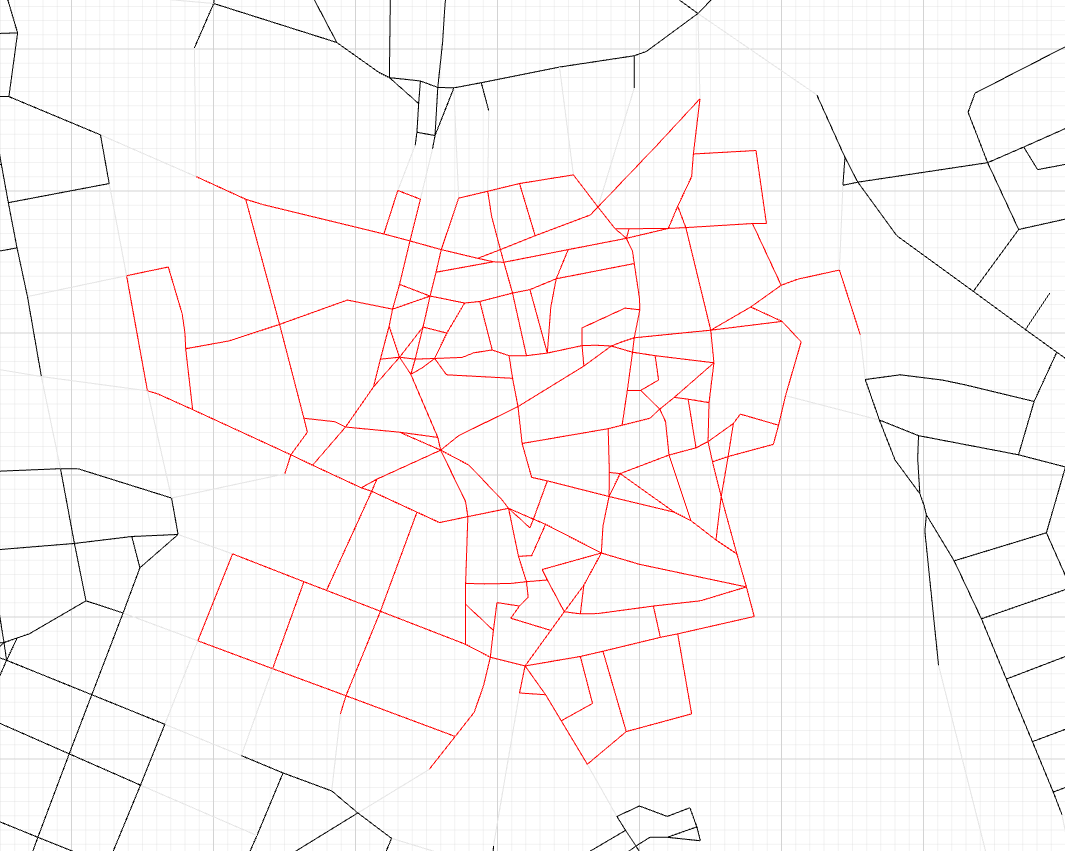
\includegraphics[width=\linewidth]{historic_district.png}
        \end{mdframed}
        \caption{Historic District of Weimar}
        \label{fig:historic_district}
    \end{subfigure}
    \par\medskip
    \begin{subfigure}[b]{0.6\textwidth}
        \begin{mdframed}[style=mdthight]
            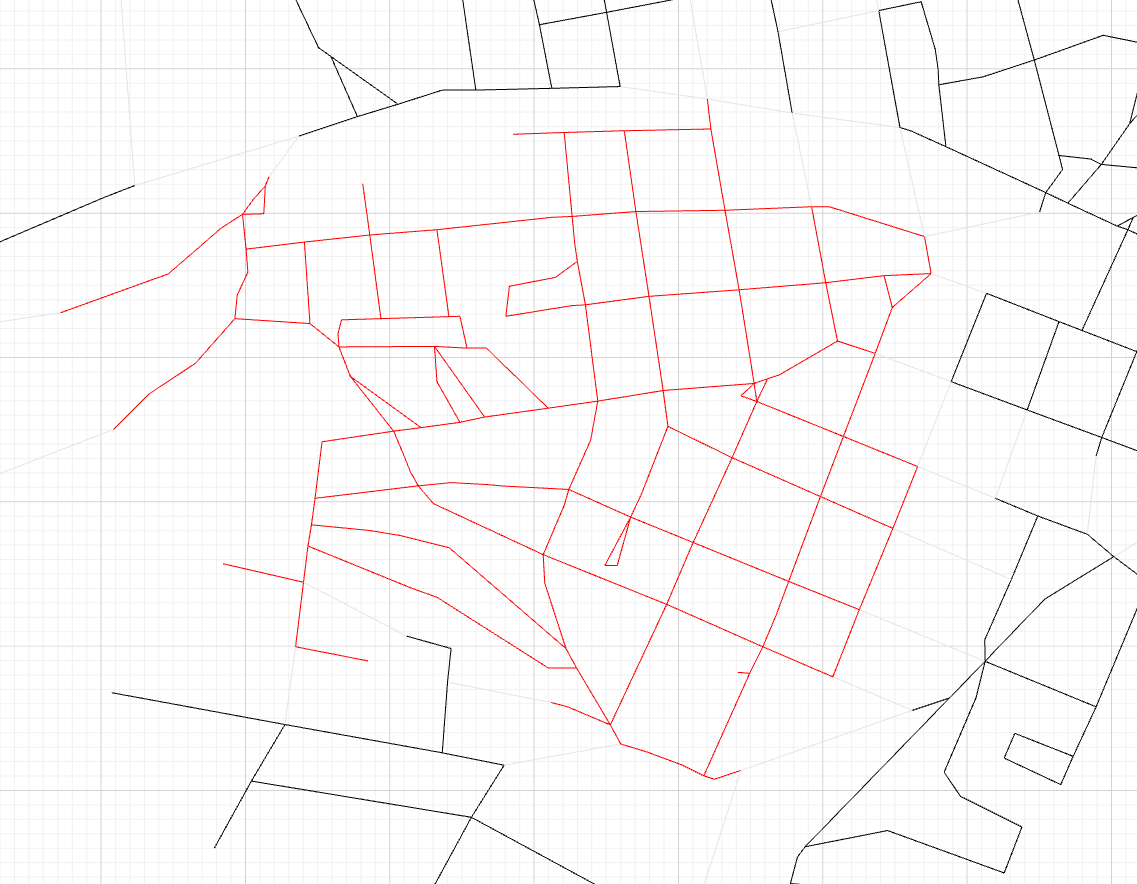
\includegraphics[width=\linewidth]{business_district.png}
        \end{mdframed}
        \caption{Business District of Weimar}
        \label{fig:business_district}
    \end{subfigure}
    \begin{subfigure}[b]{0.6\textwidth}
        \begin{mdframed}[style=mdthight]
            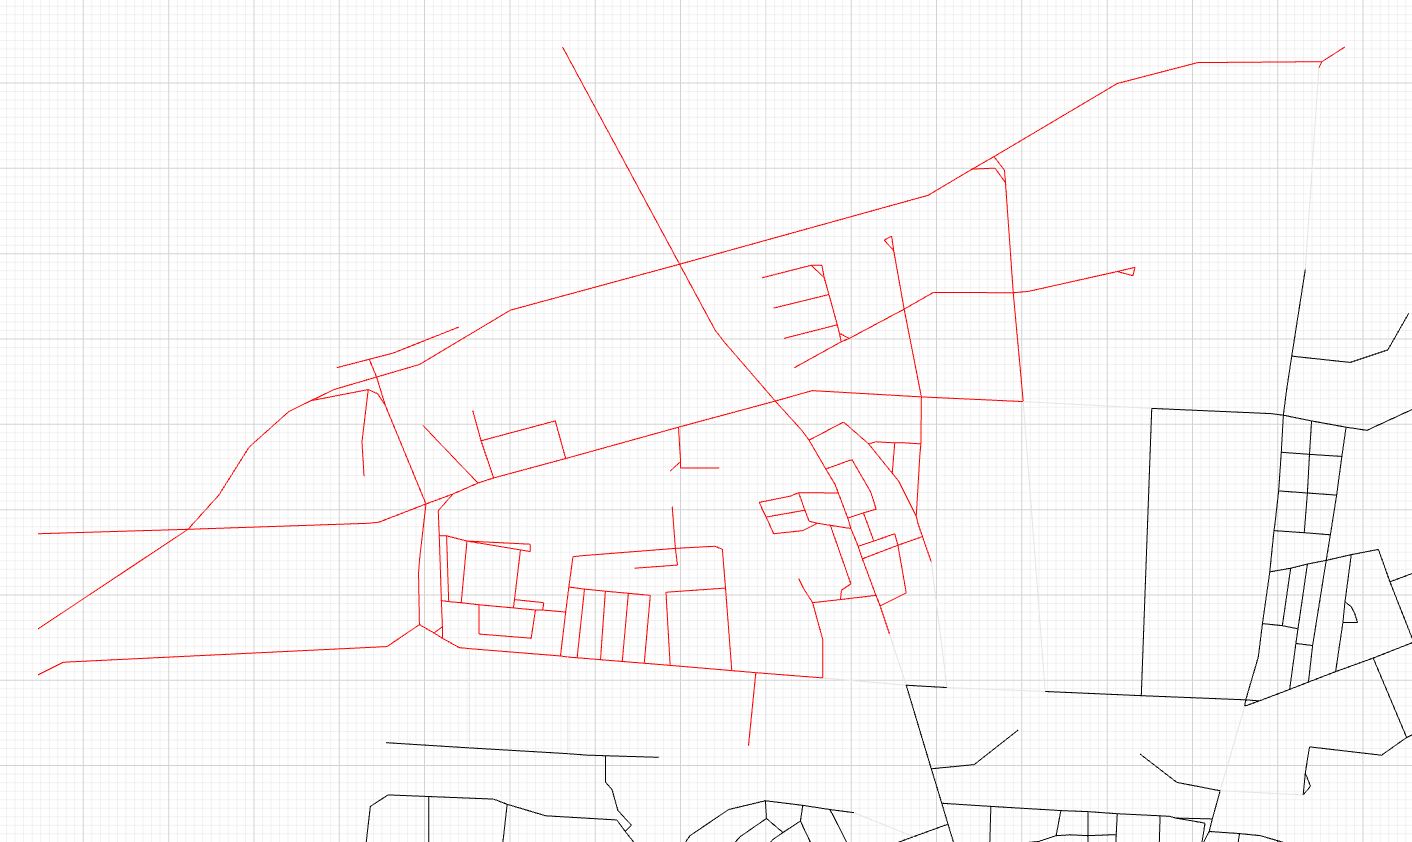
\includegraphics[width=\linewidth]{outskirts_district.png}
        \end{mdframed}
        \caption{Outskirts Area of Weimar}
        \label{fig:outskirts_district}
    \end{subfigure}
    \caption{Different areas of Weimar. Historic District (\ref{fig:historic_district}), Business District (\ref{fig:business_district}) and Outskirts Area (\ref{fig:outskirts_district})}
\end{figure}

\subsubsection{Business/Manhattan District}
\label{sec:businessDistinct}
If the relative block area (block area divided by surrounding circle) is high the given area is probably a business/Manhattan district. Most of the parameters are in the midrange. The image \ref{fig:business_district} with the measured data in table \ref{sec:ClusterAnalysisMeasurements} in column C2, is an example area of this district/area type.

\subsubsection{Outskirts Area}
\label{sec:outskits}
These areas are characterized by extreme long streets and a low connection count. As a result the density is extremely high as you can see in the example \ref{fig:outskirts_district} and the measured data in table \ref{sec:ClusterAnalysisMeasurements} in column C3. The block count is compared with a business or historic district exceptional low.